\documentclass{source/Report}

\major{电子科学与技术}
\name{朱炳昊}
\title{NA Project}
\stuid{3220105656}
\college{信息与电子工程学院}
\date{\today}
\lab{西2-213}
\course{数值分析方法}
\instructor{余官定}
\grades{}
\expname{稀疏矩阵特征值}
\exptype{大作业报告}
\partner{无}
\begin{document}
    \makecover
    \makeheader
    
        % \begin{table}[H]
        %     \centering
        %     \caption{雅可比迭代结果-4.1}
        %     \begin{tabular}{cccc}
        %     \toprule
        %     $n$ & $x_1^{(n)}$ & $x_2^{(n)}$ & $x_3^{(n)}$ \\
        %     \midrule
        %     0 & 1.25000000 & -1.33333333 & 0.20000000 \\
        %     1 & 1.63333333 & -0.85555556 & -0.11111111 \\
        %     2 & 1.43611111 & -0.81759259 & -0.04740741 \\
        %     \bottomrule
        %     \end{tabular}
        % \end{table}\par
    
    
        % \lstinputlisting[
        %     language = Python,
        %     title = {最小二乘法线性拟合代码}
        % ]{code/linear_ap.py}\par
        

%             \begin{lstlisting}[language = Verilog, title = {代码块测试(直接插入)}]
% module dffre (
%     d, en, r, clk, q
% );
%     parameter n = 1;
%     input en,r,clk;
%     input [n-1:0] d;
%     output [n-1:0] q;
%     reg [n-1:0] q;
%     always @(posedge clk) begin
%         if(r) q = {n{1'b0}};
%         else if(en) q = d;
%             else q = q;
%     end
% endmodule
%             \end{lstlisting}

%             \begin{figure}[H]
%                 \centering
%                 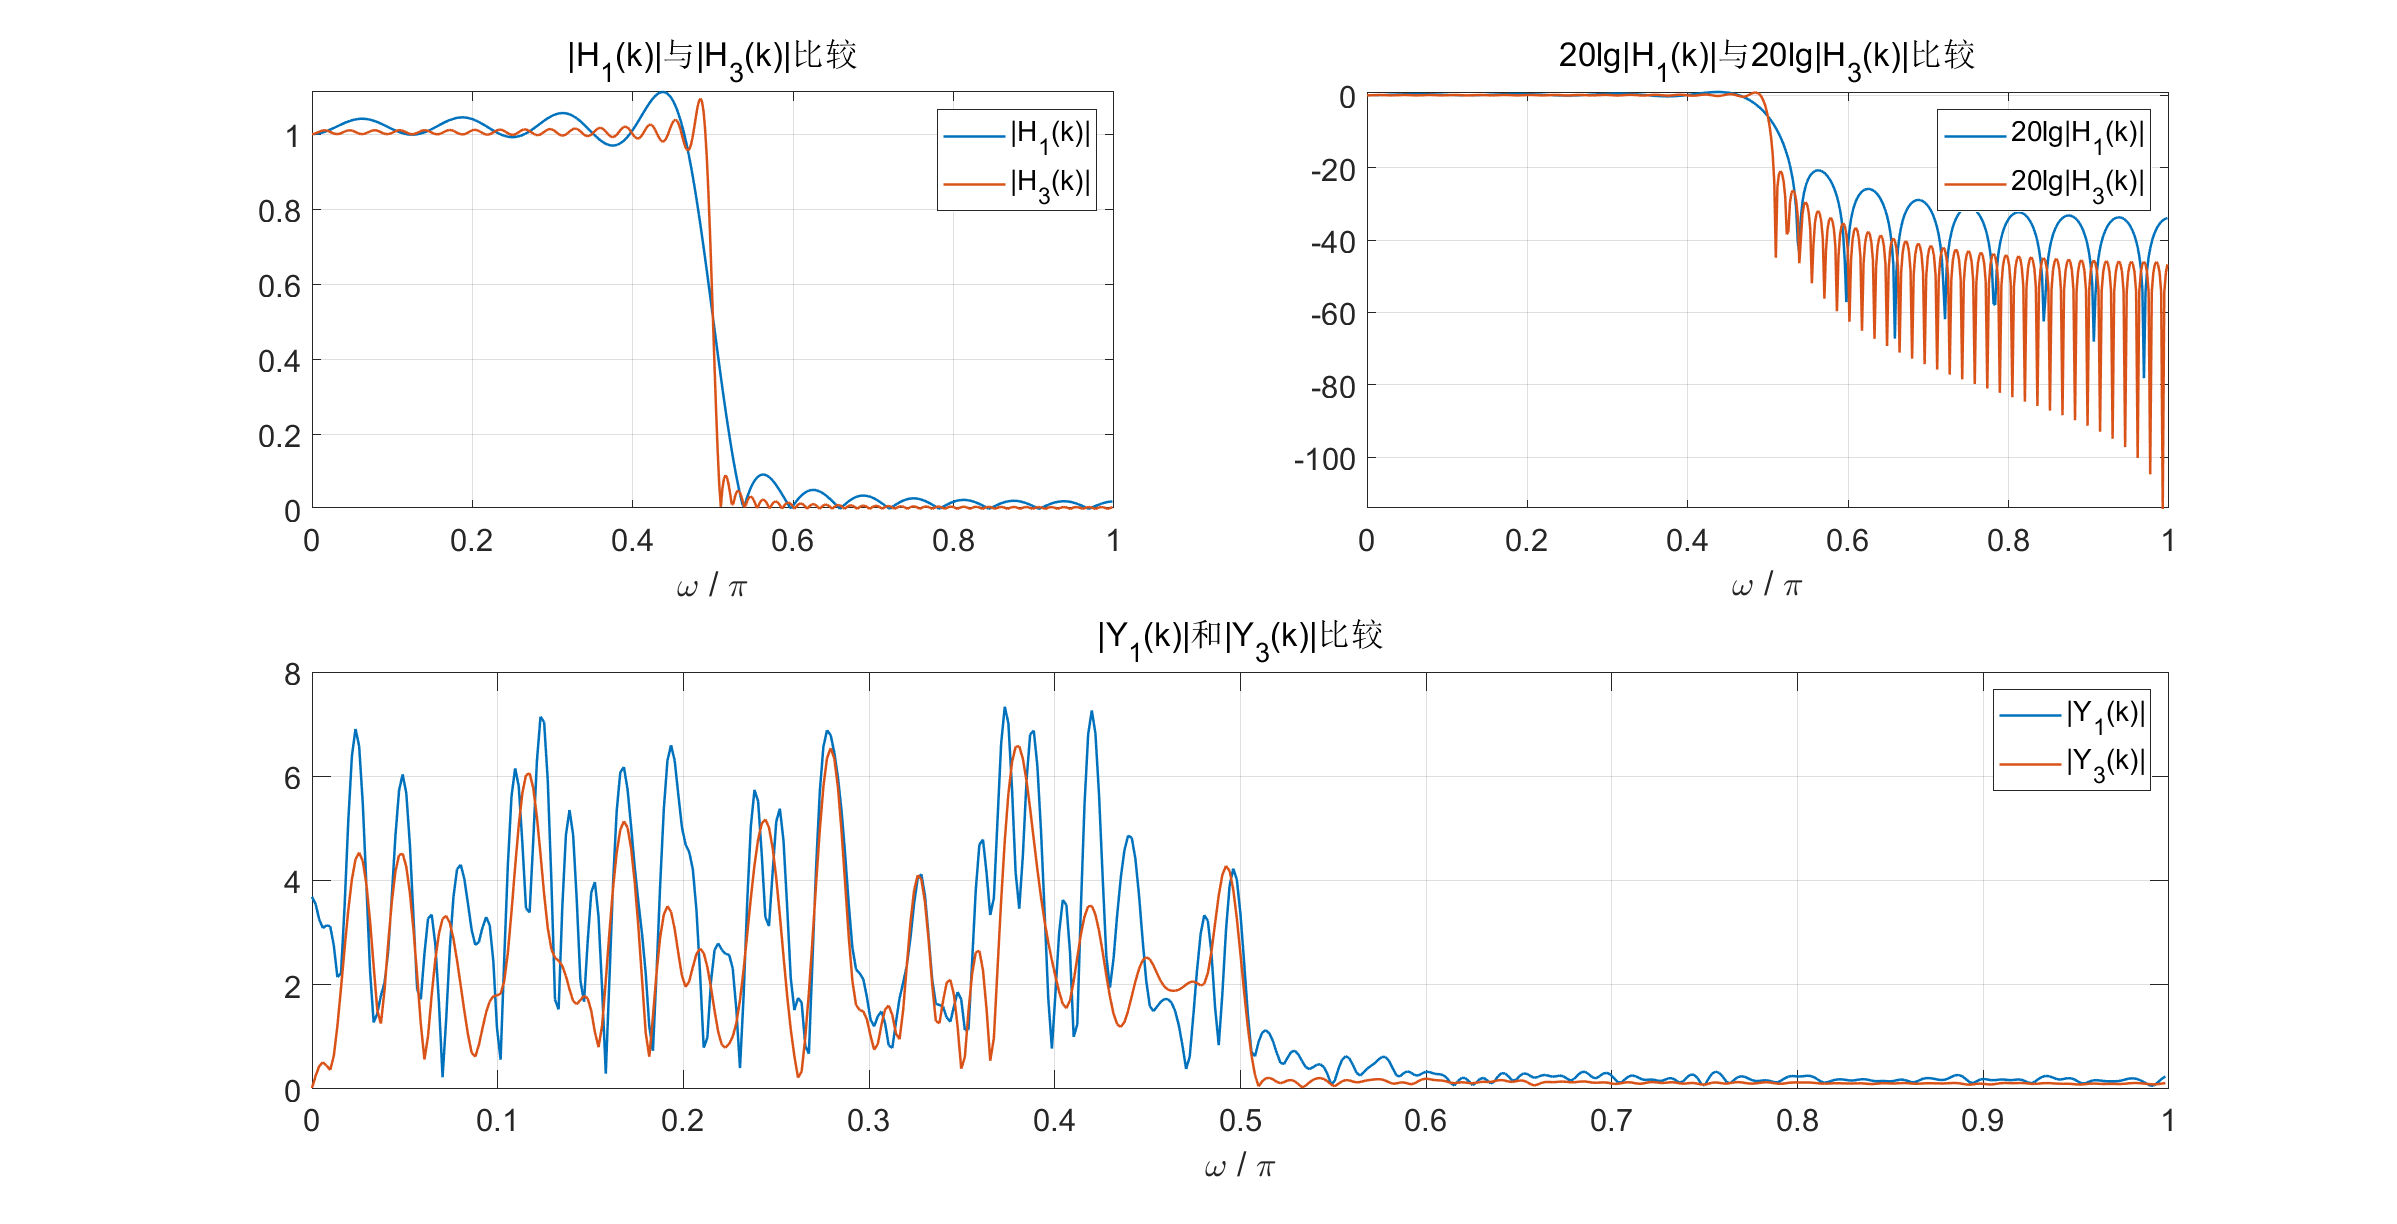
\includegraphics[width = 1\textwidth]{pic1}
%                 \caption{图片测试}
%             \end{figure}


    % \section{}
    %         \subsection{}
    %         1\footnote{测试}2
    %         \begin{table}[H]
    %             \centering
    %             \caption{表格测试}
    %             \begin{tabular}{|c|c|c|c|c|c|c|c|c|}
    %             \hline
    %             state                 & ld & st & addr{[}31:11{]} == tag & valid & dirty & l2\_ack & write\_done & nextstate                   \\ \hline
    %             \multirow{4}{*}{Idle} & 0  & 0  & -                      & -     & -     & -       & -           & Idle                        \\ \cline{2-9} 
    %                                 & 0  & 1  & -                      & -     &       & -       & -           & \multirow{3}{*}{CompareTag} \\ \cline{2-8}
    %                                 & 1  & 0  & -                      & -     &       & -       & -           &                             \\ \cline{2-8}
    %                                 & 1  & 1  & -                      & -     &       & -       & -           &                             \\ \hline
    %         \end{tabular}
    %         \end{table}
\end{document}